\documentclass[11pt]{article}
\usepackage[margin=1in]{geometry}
\usepackage{amsmath,amssymb}
\usepackage{graphicx}
\usepackage{hyperref}
\usepackage{enumitem}
\usepackage{xcolor}
\usepackage{titlesec}
\usepackage{authblk}

\hypersetup{
    colorlinks=true,
    linkcolor=blue,
    urlcolor=blue,
    citecolor=blue
}

\titleformat{\section}{\large\bfseries}{\thesection.}{0.5em}{}
\titleformat{\subsection}{\normalsize\bfseries}{\thesubsection}{0.5em}{}

\graphicspath{{figs/}}

% =====================================================================
%  纪律一：正文每个数字必须能溯源（results JSON 或所引论文），没源不写。
%  纪律二：判据在跑实验之前写死，不随结果调整。负结果如实记录。
% =====================================================================

\title{\textbf{Judge, Don't Generate: Physics-Guided Boundary Detection for Hierarchical Rollout in Frozen JEPA World Models}}
% 备选原版标题：
% When to Stop: Measured Boundaries Terminate and Re-anchor Rollouts of Frozen JEPA World Models

\author{Jiaqi Wang}
\affil{Eindhoven University of Technology \\ \texttt{j.wang11@student.tue.nl}}

\date{}

\begin{document}

\maketitle

\begin{abstract}
JEPA world models learn explicit predictive dynamics in latent space and plan by imagination, without the language supervision of vision--language--action models or the iterative action sampling of diffusion policies. Their weakness is the long horizon: rollout error compounds step by step, and the imagination of current models remains trustworthy for only tens of steps. Existing fixes train hierarchy: end-to-end multi-level architectures work but are heavy, and subgoal generators fail precisely at generation. On a frozen LeWM backbone at medium PushT distance, generated subgoals score $38.7\%$, below the $52.7\%$ of flat planning, while ground-truth subgoals reach $73.3\%$. We replace generation with judgment: a small detector network that fuses physical priors with learnable parameters reads the frozen model's own latents and decides whether the current rollout still belongs to the same dynamical phase. Training trajectories are segmented offline by measured kinematic events such as contact, release, and heading change, and these mechanically derived labels train the detector. At planning and execution time, detected boundaries govern when candidate rollouts may be truncated and when closed-loop execution re-anchors to fresh observations, clearing accumulated drift at each phase transition. Because all evaluated states lie on the model's own rollouts, unreachable fabricated subgoals cannot enter the plan. The backbone stays strictly frozen, and adapting to a new task requires only lightweight offline calibration rather than end-to-end retraining.
\end{abstract}

\section{Introduction and Related Work}

Joint-Embedding Predictive Architectures (JEPAs) learn world models by predicting the representation of the next observation rather than the observation itself~\cite{lecun2022path,assran2023ijepa}. The learned dynamics are explicit: given the current latent and an action, the model predicts the next latent, so a planner can evaluate candidate action sequences entirely in imagination. This avoids two costs: the language supervision and task demonstrations required by vision--language--action models, and the iterative sampling of diffusion policies. LeWorldModel (LeWM) shows that such a model can be trained stably end to end from pixels~\cite{lewm2026}.

\begin{figure}[!t]
\centering
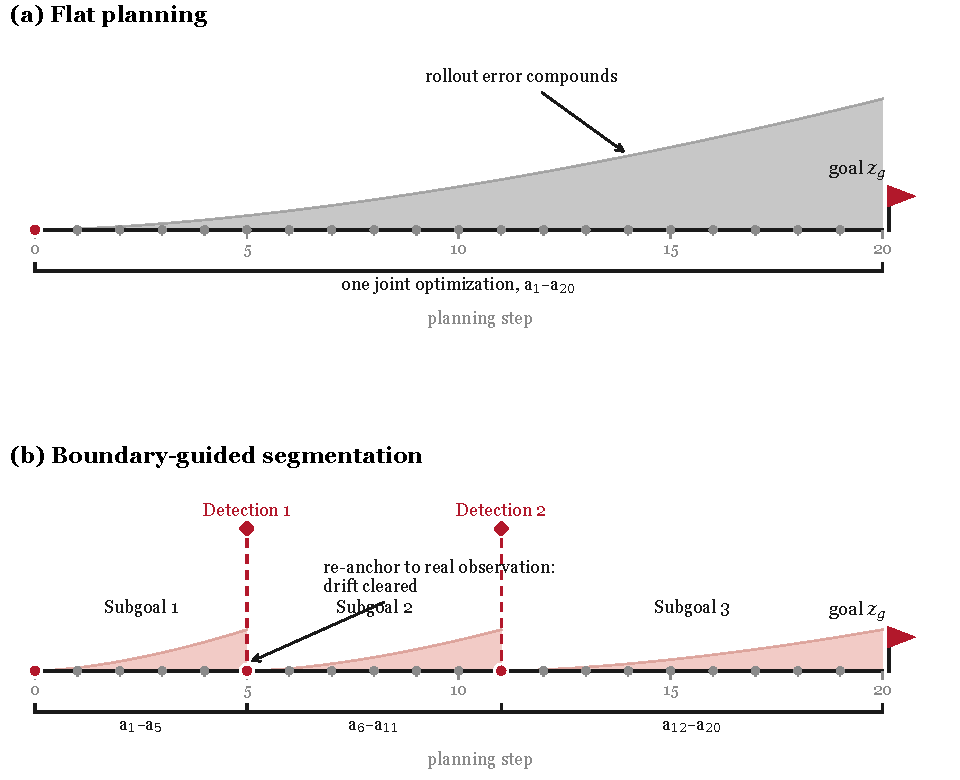
\includegraphics[width=0.96\textwidth]{rollout_flat_vs_seg_en}
\caption{Flat planning versus boundary-guided segmentation. Top: one imagined rollout covers the full horizon and all actions are optimized jointly, so rollout error compounds without reset. Bottom: the detector fires at physical phase boundaries (Detection 1 and 2, dashed lines at unequal steps); each segment takes the boundary waypoint as its subgoal and is optimized on its own, and execution re-anchors to a fresh real observation at every boundary, clearing accumulated drift. Segment lengths follow detected events, not a fixed stride.}
\label{fig:rollout}
\end{figure}

The explicit dynamics are also the weakness. Evaluating a long candidate means rolling the one-step model forward autoregressively, and prediction error compounds at every step, so the imagination of current models remains trustworthy for only tens of steps. On the frozen LeWM backbone, flat-planning success falls from $94.0\%$ at goal distance $d=25$ to $18.0\%$ at $d=75$~\cite{mindthegap2026}.

Hierarchy is the standard answer: a high level chooses intermediate targets so that every subproblem stays inside the trusted range. Behind all architectural variants, however, one question decides success or failure: where the intermediate target's latent comes from. The literature contains three answers, and each has a diagnosed failure.

\textbf{Answer 1: train the hierarchy end to end.} H-JEPA stacks levels with pooled strides of 5, 10, and 20 and trains them jointly, reporting AntMaze success rising from $18.0\%$ under flat planning to $73.3\%$~\cite{hjepa2026}. HWM learns models at several strides in a shared latent space, so that coarse predictions serve as subgoals for fine ones~\cite{hwm2026}. The gains are real, and so is the price: every new task and every new embodiment requires full end-to-end retraining.

\textbf{Answer 2: generate subgoals with a learned high level.} Mind the Gap freezes the pretrained low level and trains a macro-action encoder plus a high-level predictor on top of it~\cite{mindthegap2026}. At medium PushT distance, generated subgoals score $38.7\%$, below the $52.7\%$ of flat planning on the same frozen backbone, while ground-truth subgoals from the data reach $73.3\%$. The failure happens at generation: search selects candidates that the model scores highly but that lie off the data manifold, and the frozen low level cannot execute them. The authors' repair confines search to macro-actions encoded from real trajectories, recovering $11.3$ and $14.7$ points at the two longest distances, which amounts to abandoning generation and turning to the data.

\textbf{Answer 3: retrieve subgoals from data.} IMWM retrieves demonstrations to initialize and bias the planner's search~\cite{imwm2026}, and the confined repair above belongs to the same family. Retrieval cannot fabricate targets, but it answers only where to look nearby, never which states deserve to be waypoints. Two related lines also adjust execution pacing online: PACE finds low-speed transition points in the predicted speed profile and uses them as replanning boundaries~\cite{pace2026}, and AutoHorizon estimates the model's own reliable range from attention weights to set the execution length~\cite{autohorizon2026}.

This proposal takes the vacant fourth position: it measures dynamical boundaries instead of generating or retrieving spatial waypoints. Every task's phase structure is written in physical events such as contact, release, and heading change, and these events can be read off training trajectories mechanically. Measured boundaries decide where rollouts terminate and where execution restarts from real observations. The only training in the whole method is a lightweight calibration network that fuses physical priors with learnable parameters, supervised by labels the offline measurement produces, so what it learns is a boundary judgment that transfers across task instances rather than a brittle rule. Every decision reduces to physical invariants compared against calibrated thresholds, so the method stays auditable, and adapting to a new task takes hours without touching the frozen backbone.

The rest of the proposal states the research questions, the method, a gated work plan, and the risks and expected contributions.

\section{Research Questions and Hypotheses}

Rather than training a generative high-level policy, this proposal asks whether the benefits of hierarchy in frozen world models can be recovered purely by timing when rollouts terminate and re-anchor. We structure the investigation around four falsifiable questions and one pre-registered applicability prediction:

\textbf{RQ1 (Viability of boundary-timed replanning).} \textit{Does terminating and re-anchoring rollouts at physical phase boundaries outperform flat planning on a frozen JEPA backbone?} We test this first via an oracle ground-truth segmentation upper bound; establishing a clear margin here is the prerequisite for the entire line of inquiry.

\textbf{RQ2 (Attribution: timing vs.\ frequency, and imagination vs.\ execution).} \textit{First, does the performance gain stem from aligning replanning with physical boundaries, or merely from re-anchoring more frequently?} Measured segmentation must beat equal-stride segmentation at a strictly matched average replanning frequency. \textit{Second, where does boundary detection help most: by truncating unreliable post-boundary imagination, or by triggering closed-loop re-anchoring during execution?} We compare both mechanisms directly.

\textbf{RQ3 (Observable signatures of phase boundaries).} \textit{Which latent timescale decompositions and change-point statistics reliably capture physical transitions?} Instead of committing a priori to a single heuristic, the synthetic positive control and held-out boundary $F_1$ scores determine which timescale estimator and boundary signal advance to planning.

\textbf{RQ4 (Value of learnable calibration).} \textit{Does a lightweight learnable readout over physical features generalize better than fixed analytical thresholds?} Learnable parameters must beat the fixed-constant variant on at least two of three transfer axes (held-out noise, unseen task instances, and cross-environment transfer), or they are dropped in favor of the simpler analytical variant.

\textbf{P1 (Pre-registered applicability prediction).} While oracle spatial subgoals yield large gains on PushT ($73.3\%$ vs.\ $52.7\%$) because they supply intermediate spatial routing (\textit{where to go}), our method regulates purely the timing of horizon truncation and re-anchoring (\textit{when to stop}) while relying on the global goal latent for direction. Consequently, our method requires tasks with distinct dynamical regimes separated by clear timescale gaps. We predict substantial gains in navigation tasks with sharp topological transitions (AntMaze), and more limited gains in contact-rich manipulation (PushT, Cube) where overcoming bottleneck states requires spatial waypoint discovery rather than mere drift reset. This prediction is registered prior to comparative evaluation.

\section{Method}

The method fixes the planning protocol, the labeling mechanics, the acceptance tests, and the controlled comparison setup. The internal spectral and change-point estimators are candidate families, chosen by offline calibration before any closed-loop test.

\subsection{The boundary-guided planning protocol}

Planning proceeds as in flat Model Predictive Control (MPC) with the final goal latent $z_g$ as the sole spatial objective, modified only by how detected boundaries govern rollout evaluation and execution re-anchoring (Figure~\ref{fig:rollout}). Because truncating an imagined rollout early trades off reduced compounding error against shorter lookahead, we formulate and test two mechanisms:

\begin{enumerate}[leftmargin=*, nosep]
    \item \textbf{Mode A: Full-Horizon Imagination with Execution-Only Re-anchoring.} During planning, candidate action sequences are rolled out in imagination to the full trust cap $H_{\max}$ (e.g., tens of steps) and scored by their terminal latent distance to $z_g$, preserving maximum lookahead for navigating non-convex obstacles. Boundary detection operates strictly during closed-loop execution: instead of executing a fixed stride $k$, execution halts when the detector identifies a phase boundary in the real observation stream (or reaches $H_{\max}$), and planning restarts from the fresh observation.
    \item \textbf{Mode B: Boundary-Truncated Imagination with Normalized Scoring.} During planning, if a candidate rollout triggers the detector at step $h_b < H_{\max}$, the rollout terminates immediately at $h_b$ on the premise that post-boundary predictions (e.g., after an unmodeled contact or sharp turn) are unreliable. To prevent horizon-length bias when comparing candidates that terminate at different steps $h_b$, trajectories are scored by their step-normalized progress rate toward the goal latent, $\big(\|z_t - z_g\|_2 - \|z_{t+h_b} - z_g\|_2\big)/h_b$, alongside discounted terminal distance as an ablation. Execution follows the same event-triggered re-anchoring as Mode A.
\end{enumerate}

Testing Mode A against Mode B directly answers whether post-boundary latent predictions in frozen JEPA models provide useful lookahead or detrimental noise.

\subsection{Measuring time scales}

To distinguish fast transient fluctuations from slow task progression, the detector requires a timescale decomposition of the latent space. We evaluate four candidate estimators: \textbf{(1)} Autocorrelation integrals with initial-positive-sequence truncation~\cite{geyer92}, which are simple but sensitive to the encoder's coordinate basis. \textbf{(2)} Eigenvalues of data-fitted linear operators converted to timescales via $\tau = -1/\ln|\lambda|$, using Dynamic Mode Decomposition (DMD) and Extended DMD~\cite{dmd,koopman_edmd,arbabi17}, which are invariant to latent basis rotations. \textbf{(3)} Slow Feature Analysis (SFA), which extracts the slow subspace directly~\cite{sfa}. \textbf{(4)} The Jacobian spectrum of the learned one-step predictor evaluated at training states, providing a model-side reading independent of trajectory policy statistics. Two validation gates apply before any decomposition is trusted: two independent estimators must agree on the spectral gap, and each extracted scale group must decode its corresponding physical factors under linear probing, otherwise the frozen backbone is declared unfit.

\subsection{Detecting boundaries}

Given the extracted slow and fast subspaces, we evaluate three candidate boundary signals: \textbf{(1)} Energy switching: the fraction of latent increment energy carried by a specific scale group departs from its within-segment baseline, following the classic change-point detection tradition~\cite{page1954cusum,killick2012pelt,adams2007bocpd}. \textbf{(2)} Direction rotation: the cosine similarity of consecutive increments within the slow subspace drops sharply, capturing geometric transitions (such as corridor corners in AntMaze) where kinetic energy remains constant while heading flips. \textbf{(3)} Operator shift: a local linear propagator fitted over a sliding window exhibits a jump in its spectral distance~\cite{dmd,arbabi17}, a direct reading of a switch in the local dynamics. For tasks exhibiting diffuse transitions, we include an unsupervised soft phase-clustering fallback. The synthetic positive control and held-out $F_1$ scores select the operational signal.

\subsection{The physics-guided learnable detector}

To generalize across task instances without hallucinating boundaries, the detector is structured as a strict two-stage hybrid architecture:
\begin{enumerate}[leftmargin=*, nosep]
    \item \textbf{Frozen spectral measurement:} Timescale constants and slow/fast subspace projection matrices are measured offline via Sec.~3.2 and remain strictly frozen.
    \item \textbf{Learnable calibration head:} The network receives only low-dimensional, physically interpretable invariants computed on latent increments (scale-group energy shares, slow-subspace directional shifts, and local operator distances). A compact parameterization learns the readout weights and calibration constants (window decay factors, sensitivity exponents, and decision thresholds), supervised offline by mechanically derived event labels.
\end{enumerate}
Three rules enforce physical grounding: labels come strictly from offline kinematic measurements rather than self-training; spectral bases are measured rather than fitted; and the functional form of the physical invariants cannot be altered by gradient updates. The learnable and fixed-constant variants are compared head to head, and learning that buys no measurable transfer gain is dropped.

\subsection{Labels, acceptance criteria, and controlled comparison}

All validation criteria are locked prior to closed-loop experimentation. Reference boundary labels are derived mechanically from trajectory kinematics (contact-force impulses and release events in manipulation; velocity inflections and topological cell transitions in navigation), never hand-annotated, and verified visually on 10 sampled trajectories per environment. Detector acceptance is scored by held-out event $F_1$ within a strict step tolerance under three mandatory sanity controls: measured segmentation must outperform equal-stride segmentation, a detector with shuffled thresholds must collapse to chance, and a collapsed constant latent must yield zero boundaries.

The closed-loop comparison evaluates four setups across Mode A and Mode B: \textbf{(1) Flat planning}, \textbf{(2) Equal-stride segmentation}, \textbf{(3) Measured segmentation}, and \textbf{(4) Oracle ground-truth segmentation} as the upper bound. Experiments run on AntMaze, PushT, and Cube~\cite{hjepa2026} at goal distances $d \in \{25, 50, 75\}$ under the Mind the Gap evaluation protocol~\cite{mindthegap2026}, logging success rate, boundary $F_1$, and wall-clock planning compute.

\section{Staged Work Plan and Decision Gates}

The project follows a gated execution plan where each stage acts as a falsification filter before downstream compute is committed. Negative results at any gate are documented and reported as empirical findings.

\textbf{Stage 0: Baseline verification.} Reproduce flat-planning baselines on all three environments across $d \in \{25, 50, 75\}$ using released checkpoints and quantify multi-seed variance. \textit{Gate:} Resolve any discrepancy with published baselines before proceeding.

\textbf{Stage 1: Spectral audit and pre-registration.} Measure the latent timescale spectrum on each environment's training dataset, verify subspace semantics via linear probes, and formally lock the applicability prediction (P1). \textit{Gate:} If no environment exhibits a separable spectral gap, report the representation diagnosis directly.

\textbf{Stage 2: Automated kinematic labeling.} Derive reference boundary labels mechanically from trajectory kinematics and spot-check 10 trajectories per environment by eye. \textit{Gate:} Refine kinematic threshold heuristics if visual alignment fails.

\textbf{Stage 3: Detector selection and calibration.} Validate all timescale (Sec.~3.2) and boundary (Sec.~3.3) candidates on a synthetic switching linear dynamical system first, then calibrate and score held-out $F_1$ on real trajectories. \textit{Gate:} Only estimators passing the synthetic control and mandatory sanity checks advance to planning.

\textbf{Stage 4: Closed-loop planning attribution (RQ1 \& RQ2).} Run the four planning setups across three environments and three goal distances, comparing both Mode A (execution-only re-anchoring) and Mode B (imagination truncation + execution re-anchoring). The Oracle ground-truth setup runs first to verify the viability ceiling (RQ1), followed by the matched-frequency comparison between Measured and Equal-Stride segmentation (RQ2).

\textbf{Stage 5: Generalization and ablation (RQ4).} Train the learnable calibration head and evaluate against the fixed-constant analytical variant across held-out observation noise, unseen task layouts, and cross-environment transfer. Drop learnable parameters if transfer gains are not statistically significant.

\textbf{Stage 6: Fast-adaptation benchmark.} Package the pipeline into an automated calibration script, execute a blind re-calibration on a held-out task variant, and record wall-clock runtime to test the hours-not-training-runs adaptation claim.

\section{Risks and Limitations}

\textbf{Generalization vs.\ overfitting.} A rigid analytical rule book recognizes only transition magnitudes seen during calibration. Conversely, an unconstrained neural network risks overfitting to spurious latent artifacts. By fixing the spectral projection and invariant forms via physical priors while calibrating only the low-dimensional decision head, the detector can generalize across new boundary configurations governed by the same physics. Generalization is tested across three transfer axes in Stage 5.

\textbf{Single-segment vs.\ full-horizon lookahead.} In Mode B, truncating imagination at the first boundary prevents compounding error from corrupting the rollout, but restricts lookahead in non-convex environments (e.g., U-turns in AntMaze where moving toward a corner temporarily increases Euclidean distance to the goal). Evaluating Mode A alongside Mode B directly mitigates this risk: if full-horizon imagination is required for topological routing while boundary-triggered re-anchoring stabilizes execution, Mode A isolates exactly that benefit.

\textbf{Task applicability.} Boundary-timed replanning requires a usable gap in the task's timescale spectrum and rewards drift removal over spatial subgoal discovery. By testing AntMaze alongside PushT and Cube under a pre-registered hypothesis (P1), positive gains in navigation and limited gains in manipulation both mark where timing-based hierarchy suffices.

\textbf{Backbone ceiling.} All claims are conditional on a frozen backbone whose latent space encodes the task's physical state. The linear probing gate in Stage 1 filters out degenerate backbones; failures from visual domain shift at the encoder level are out of scope.

\section{Expected Contributions}

\textbf{Deconstructing hierarchy in world models.} We test the hypothesis that a primary load-bearing mechanism of hierarchical planning in frozen JEPA models is rollout termination timing and closed-loop re-anchoring rhythm, disentangling temporal pacing from spatial subgoal generation.

\textbf{The measurement route.} We complete the taxonomy of hierarchical world model planning (end-to-end training, subgoal generation, data retrieval, and boundary measurement) with a controlled comparison of both truncation and re-anchoring mechanisms.

\textbf{Physics-guided boundary calibration.} We introduce an auditable detector architecture that bridges analytical change-point rules and black-box classifiers, adapting frozen world models to new tasks via lightweight offline calibration.

\bibliographystyle{plain}
\bibliography{refs}

\end{document}